\documentclass[12pt, a4paper]{article}
\usepackage[francais]{babel}
\usepackage{caption}
\usepackage{graphicx}
\usepackage[T1]{fontenc}
\usepackage{listings}
\usepackage{geometry}
\usepackage[colorlinks=true,linkcolor=black,anchorcolor=black,citecolor=black,filecolor=black,menucolor=black,runcolor=black,urlcolor=black]{hyperref}

% \usepackage{mathpazo} --> Police à utiliser lors de rapports plus sérieux

\usepackage{fancyhdr}
\pagestyle{fancy}
\lhead{}
\rhead{}
\chead{}
\rfoot{\thepage}
\lfoot{Martin Baumgaertner}
\cfoot{}

\renewcommand{\headrulewidth}{0.4pt}
\renewcommand{\footrulewidth}{0.4pt}

\begin{document}
\begin{titlepage}
	\newcommand{\HRule}{\rule{\linewidth}{0.5mm}} 
	\center 
	\textsc{\LARGE iut de colmar}\\[6.5cm] 
	\textsc{\Large saé - concevoir un réseau multi-sites}\\[0.5cm] 
	\textsc{\large Année 2022-23}\\[0.5cm]
	\HRule\\[0.75cm]
	{\huge\bfseries Partie services réseaux}\\[0.4cm]
	\HRule\\[1.5cm]
	\textsc{\large martin baumgaertner}\\[6.5cm] 

	\vfill\vfill\vfill
	{\large\today} 
	\vfill
\end{titlepage}
\newpage
\tableofcontents
\newpage
\section{Introduction}
Le but principale de cette SAÉ fût bien sûr de développer un réseau informatique
qui s'étend sur plusieurs sites. Pour cela, mes camarades ont utilisés des protocoles
de routage propore à leurs besoins. Pour ma part, j'ai choisi de mettre en place
les services réseaux. Donc bien entendu, les protocoles et technologies utilisés
ont été différentes. Je vais donc vous expliquer à travers ce rapport, comment
j'ai mis en place les différents services réseaux nécessaires au projet,
à savoir ; les DNS, le serveur DHCP, le serveur WEB et le serveur mail.


\section{les DNS}
    \subsection{Explication}
    Pour la mise en place des DNS, j'ai utilisé le logiciel Bind9 
    le logiciel libre Bind9, présent exclusivement sur Linux. J'ai fait 
    le choix de ce logiciel car c'était celui que nous utilisions pendant
    les cours de M. BINDEL en début d'année, mais également celui que nous 
    utilisions en TP l'an dernier avec Mme LACROIX. Il y aura donc deux DNS, 
    respectivement nommés de la manière suivante \texttt{ns1.ucexchange.com}
    et \texttt{ns2.ucexchange.com}. 


    \subsection{Le DNS primaire}
    
    \subsubsection{Zone de résolution directe}
    Pour la mise en place du DNS primaire, j'ai crée un contenur LXC sous
    ubuntu. J'y ai donc installé Bind9 avec la commande suivante : 
    \texttt{sudo apt install bind9}. Puis, j'ai configuré les fichiers
    de configuration de bind9 qui se trouvent tous dans le répertoire 
    \texttt{/etc/bind/}. Pour commencer, il faut déclarer une zone. 
    Pour ce faire, il faut éditer le fichier named.conf.local. Voici la
    configuration que j'ai mis dans ce fichier :

    \begin{figure}[h]
		\centering
		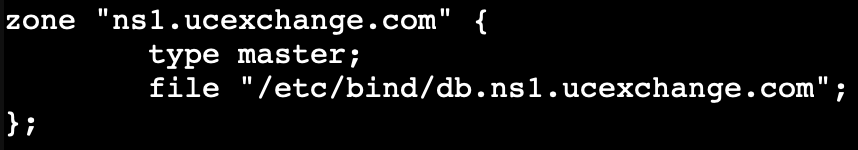
\includegraphics[width=0.8\textwidth]{img/zone1.png}
		\caption{Déclaration de la zone de résolution directe}
		\label{fig:zone1}
	\end{figure}
    
    Cette déclaration permet de dire au bind9 où il doit chercher le
    fichier de zone de résolution directe. Ce fichier se trouve dans le
    répertoire \texttt{/etc/bind/} et s'appelle \texttt{db.ns1.ucexchange.com}
    que nous allons voir ci-dessous : 
    \newpage

    \begin{figure}[h]
		\centering
		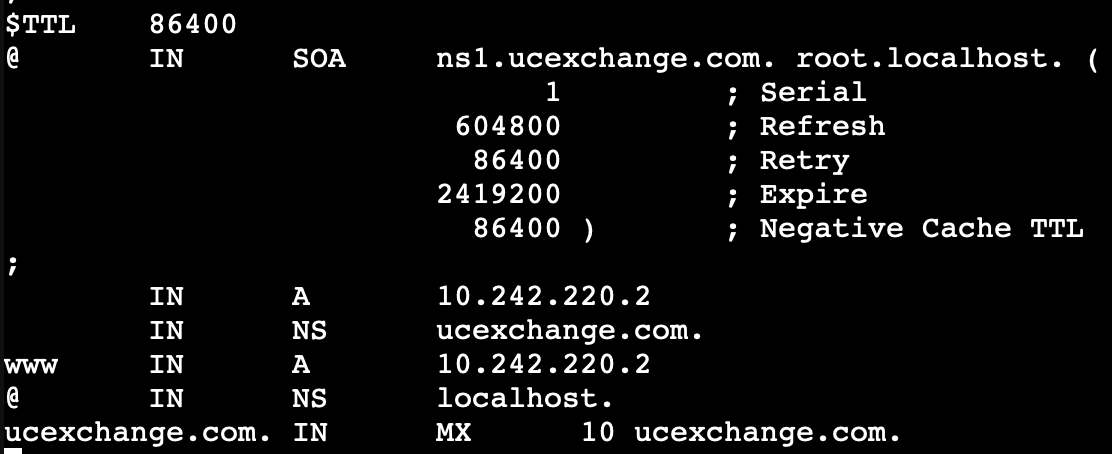
\includegraphics[width=0.9\textwidth]{img/zone1-db.png}
		\caption{Configuration de la zone de résolution directe}
		\label{fig:zone1-db}
	\end{figure}
    Voici donc le fichier de configuration pour la résolution directe de mon 
    premier DNS. Je vais vous expliquer les lignes de manière détaillée ci-après :\\

    \begin{itemize}
        \item \textbf{\$TTL 86400} définit le Time To Live par défaut pour les enregistrements dans cette zone en secondes. Cela signifie que les informations contenues dans ces enregistrements ne seront pas mises à jour plus souvent que toutes les 86400 secondes (24 heures).\\
        \item \textbf{@ IN SOA ns1.ucexchange.com. root.localhost.} définit le début de l'enregistrement de début de zone (SOA). Le caractère \textbf{@} représente le nom de domaine lui-même, ici \textbf{ucexchange.com}. \textbf{SOA} indique que cet enregistrement est un enregistrement \textbf{SOA} et \textbf{ns1.ucexchange.com.} est le nom du serveur d'origine pour cette zone.\textbf{root.localhost.} est l'adresse e-mail du responsable technique pour cette zone.\\
        \item \textbf{IN NS ucexchange.com.} définit un enregistrement \textbf{NS} (Name Server) pour le nom de domaine @, indiquant que le serveur de nom \textbf{ucexchange.com} est responsable de la résolution des noms pour ce domaine.\\
        \item  \textbf{www IN A 10.242.220.2} définit une adresse IPv4 pour le nom de domaine www.\\
        \item  \textbf{ucexchange.com. IN MX 10 ucexchange.com.} définit un enregistrement MX (Mail Exchange) pour le nom de domaine "ucexchange.com." indiquant que le serveur de messagerie "ucexchange.com" est responsable de la gestion des courriels pour ce domaine.\\
    \end{itemize}
    \newpage

    \subsubsection{Zone de résolution inverse}
    Pour la zone de résolution inverse, j'ai utilisé le même principe que pour
    la zone de résolution directe. Mais il faut déclarer la zone et son fichier. 
    Voici comment j'ai déclaré la zone de résolution inverse dans le fichier
    \texttt{named.conf.local} :
    \begin{figure}[h]
		\centering
		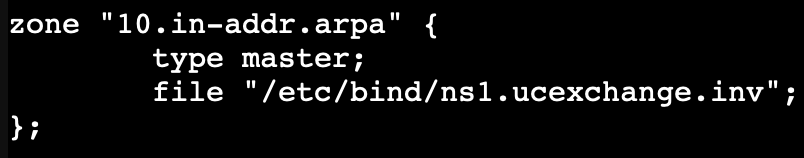
\includegraphics[width=0.9\textwidth]{img/zone-inv.png}
		\caption{Déclaration de la zone de résolution indirecte}
		\label{fig:zone-inv}
	\end{figure}

    Comme avant, je viens défnir dans quel fichier sera enregistré ma
    configuration de zone indirecte.\\
    
    La spécitié de la résolution indirecte
    est qu'on va donc mettre à l'envers les adresses IP dans les fichiers 
    de configuration comme vous pouvez le constater ci-dessous : 

    \begin{figure}[h]
		\centering
		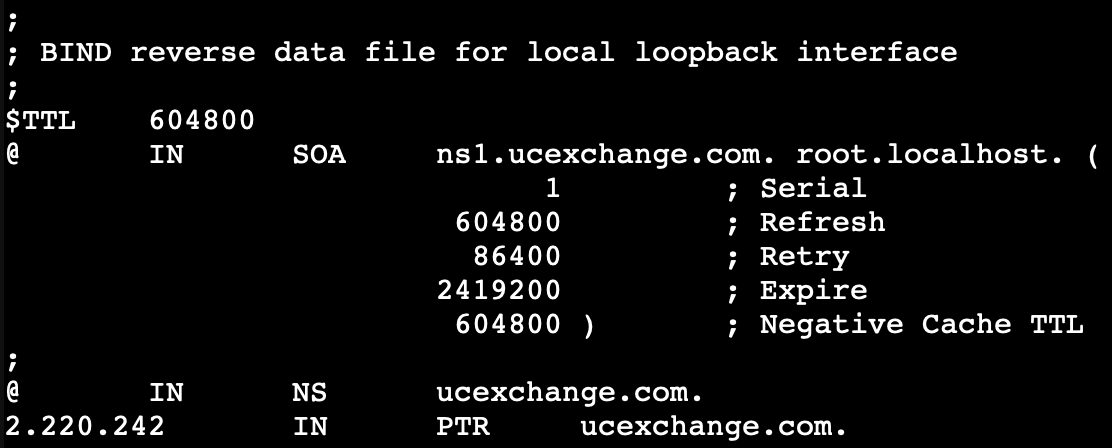
\includegraphics[width=0.9\textwidth]{img/ns1-inv.png}
		\caption{Configuration de la zone de résolution indirecte}
		\label{fig:ns1-inv}
	\end{figure}

    \begin{itemize}
        \item le terme \texttt{IN PTR} signifie que c'est une zone de résolution indirecten elle permet de faire l'inverse que la zone de résolution directe. Cette dernière va permettre de transformer un nom en adresse IP. Tandis que la zone de résolution inverse va permettre de transformer une adresse IP en nom. 
    \end{itemize}

    \newpage
    \subsubsection{Test du premier DNS}

    Nous pouvons tester le dns primaire, en prenant une machine test que j'ai 
    crée exprès pour l'occasion. Je me suis mis dans le même réseau que le DNS 
    primaire et quand j'éffectue la commande \texttt{nslookup ns1.ucexchange.com}
    j'ai bien le retour attendu : 

    \begin{figure}[h]
		\centering
		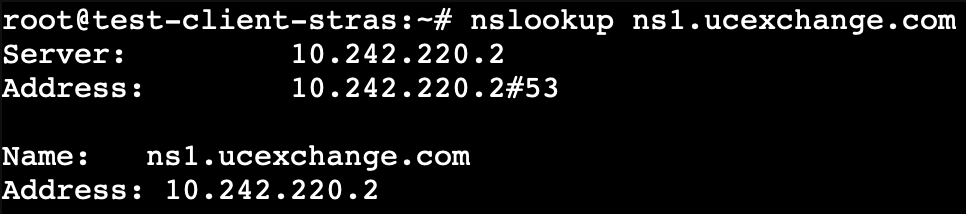
\includegraphics[width=0.9\textwidth]{img/ns-ns1.png}
		\caption{Retour de la commande \texttt{nslookup ns1.ucexchange.com}}
		\label{fig:ns1-ns}
	\end{figure}

    Nous constatons que je récupère bien l'adresse IP du DNS primaire avec son nom
    associé.\\





    \subsection{Le DNS secondaire}
    \subsubsection{Zone de résolution directe}

    Le but du DNS secondaire et qu'il hérite du premier DNS. Donc
    j'ai laissé une configuration assez minimale pour le DNS secondaire qui
    est \texttt{ns2.ucexchange.com}. J'ai donc redéclaré la zone
    exactement de la même manière que pour le premier DNS : 

    \begin{figure}[h]
		\centering
		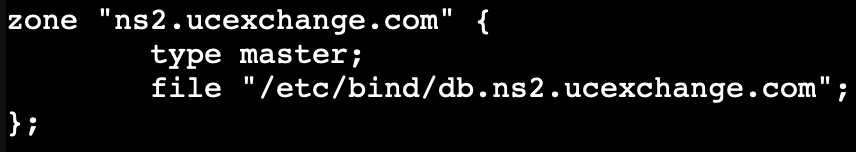
\includegraphics[width=0.9\textwidth]{img/ns2-de.png}
		\caption{Déclaration de la zone de résolution directe}
		\label{fig:ns2-de}
	\end{figure}

    \newpage

    Pour la zone de résolution directe du deuxième DNS, j'ai laissé 
    par défaut les valeurs, car comme je l'ai expliqué plutôt, le DNS secondaire
    hérite du DNS primaire :\\

    \begin{figure}[h]
		\centering
		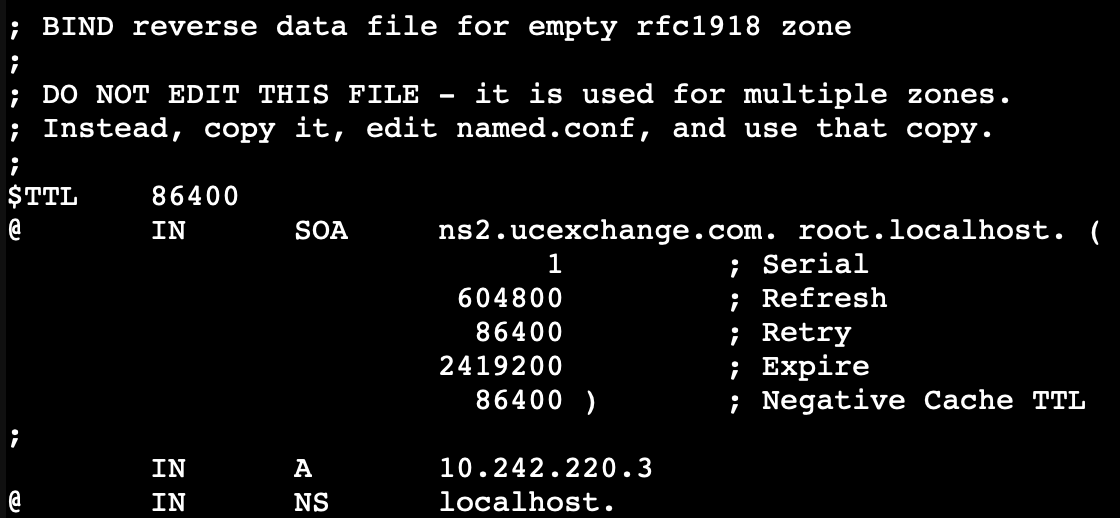
\includegraphics[width=0.9\textwidth]{img/ns2-ex.png}
		\caption{Configuration du DNS secondaire}
		\label{fig:ns2-ex}
	\end{figure}
    
    L'explication des lignes de configuration du premier DNS est toujours valable
    pour le DNS secondaire car c'est la même chose. 

    \subsubsection{Zone de résolution inverse}

    Pöur la zone de résolution inverse du DNS secondaire, j'ai repris exactement 
    les mêmes paramètres que pour le premier DNS car ici, le but n'était pas de 
    faire une résolution inverse très compliqué. 

    \subsubsection{Test du DNS secondaire}
    Comme pour le DNS primaire nous pouvons effectuer la commande 
    \texttt{nslookup ns2.ucexchange.com} pour voir si le DNS secondaire est
    bien en place. Voici le résultat :

    \begin{figure}[h]
		\centering
		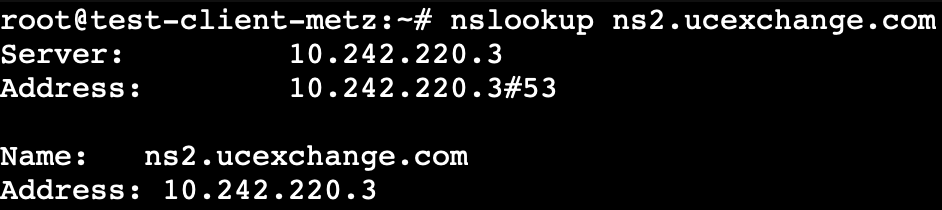
\includegraphics[width=0.7\textwidth]{img/nslook.png}
		\caption{Test du DNS secondaire}
		\label{fig:nslook}
	\end{figure}



\section{le DHCP}
    \subsection{Explication du DHCP}
    Un serveur DHCP (Dynamic Host Configuration Protocol) est utilisé 
    pour attribuer des adresses IP à des ordinateurs et d'autres dispositifs 
    sur un réseau. Il joue un rôle clé dans la configuration automatique des 
    paramètres réseau pour les ordinateurs et autres dispositifs connectés au 
    réseau.\\

    Lorsqu'un ordinateur ou un autre dispositif se connecte à un réseau, 
    il envoie une requête DHCP pour demander une adresse IP. Le serveur DHCP 
    répond en attribuant une adresse IP disponible à ce dispositif, ainsi que 
    d'autres paramètres de configuration réseau tels que le masque de 
    sous-réseau, la passerelle par défaut et les serveurs DNS.\\

    L'utilisation d'un serveur DHCP simplifie la gestion des adresses IP 
    sur un réseau car il automatise la distribution des adresses IP, ce 
    qui évite les erreurs de configuration manuelle et rend plus facile 
    le suivi de l'utilisation des adresses IP sur le réseau.\\

    En plus de cela, un serveur DHCP permet de configurer de manière 
    centralisée les paramètres réseau pour les dispositifs sur le réseau. 
    Cela signifie que vous pouvez facilement apporter des modifications aux 
    paramètres réseau pour de nombreux dispositifs en une seule étape, plutôt 
    que de devoir les configurer manuellement sur chaque dispositif 
    individuellement.\\
    
    J'ai choisi d'utiliser le logiciel \texttt{isc-dhcp-server}, encore une fois présent sur Linux.
    Pour pouvoir le configurer il faut l'installer via la commande suivante : 
    \texttt{apt-get install isc-dhcp-server}

    \section{Mise en place du DHCP}
    Une fois installé la configuration est assez simple, il suffit de déclarer 
    plusieurs paramètres pour que le serveur DHCP fonctionne. Par exemple, le 
    serveur DNS, les adresses de gateway, les adresses IP à attribuer, etc.\\

    \newpage
    Voici la configuration que j'ai pu faire, à chaque fois en déclarant
    des plages d'adresses IP différentes pour les différents Vlans de chaque sites
    (Strasboug et Metz).

    \begin{figure}[h]
		\centering
		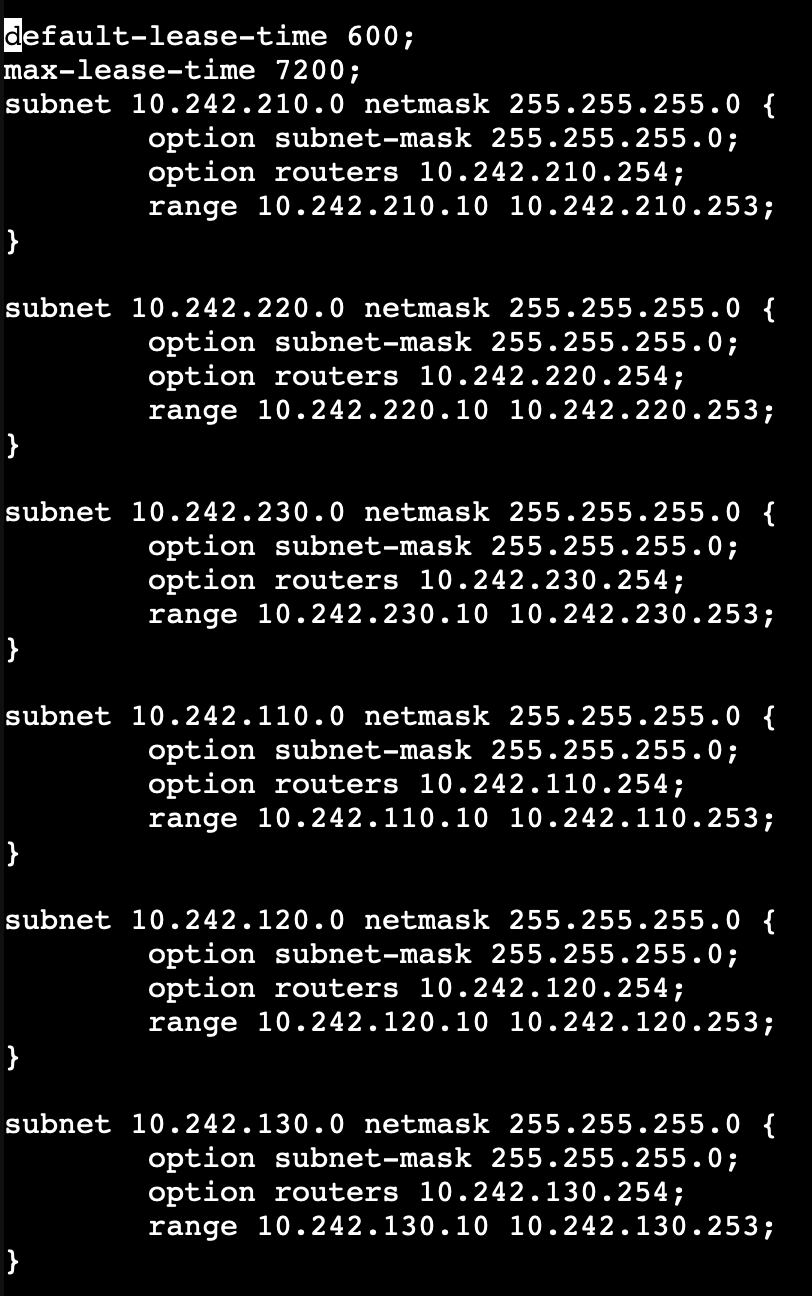
\includegraphics[width=0.5\textwidth]{img/dhcp.png}
		\caption{Configuration du serveur DHCP}
		\label{fig:dhcp}
	\end{figure}

    Nous y voyons donc plusieurs paramètres. Voici quelques explications :\\
    \begin{itemize}
        \item \texttt{default-lease-time} : permet de déclarer le temps d'attribution d'une IP
        \item \texttt{max-lease-time} : permet de déclarer le temps maximum d'attribution d'une IP
        \item \texttt{option routers} : permet de déclarer les adresses de gateway
        \item \texttt{option subnet-mask} : permet de déclarer le masque de sous-réseau
        \item \texttt{range} : permet de déclarer les plages d'adresses IP à attribuer
    \end{itemize}

    \subsubsection{test du serveur DHCP}
    Pour pouvoir vérifier que mon serveur DHCP fonctionne, j'ai crée des VM 
    en utilisant le réseau du serveur DHCP, et nous pouvons constater que 
    mes VM obtiennent bien une adresse IP automatiquement : 

    \begin{figure}[h]
		\centering
		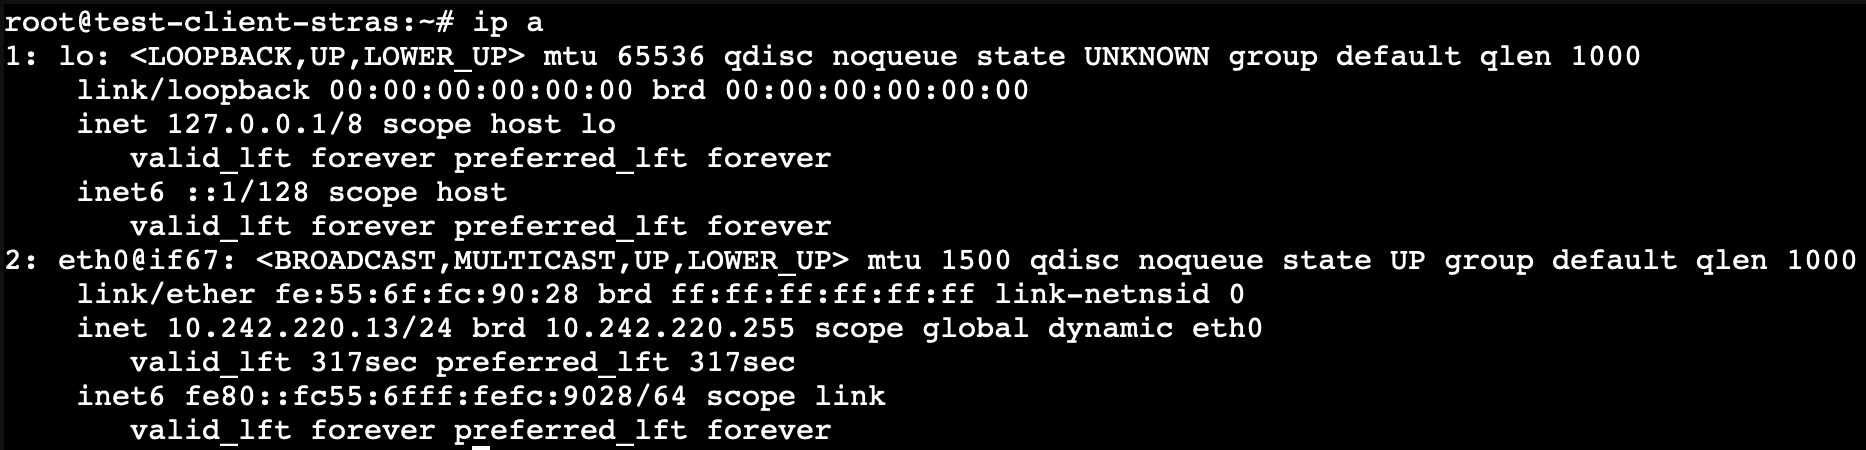
\includegraphics[width=0.9\textwidth]{img/test-dhcp.png}
		\caption{Test du serveur DHCP}
		\label{fig:test-dhcp}
	\end{figure}

    Nous avons bien une adresse IP en 10.242.220.XX

\section{Le serveur WEB}
Pour la mise en place du serveur Web j'ai tout simplement utilisé Apache2.
Pour l'installer il suffit d'utiliser la commande suivante \texttt{apt-get install apache2}.
Une fois installé, j'ai laissé par défaut la page car le but était ici de 
pouvoir effectuer une requête \texttt{ping}. Mais aussi, le but était de pouvoir
atteindre le serveur web avec le DNS de l'entreprise. Donc nous pouvons 
faire un ping vers le nom de domaine du serveur et nous avons bien une réponse 
comme le démontre la capture d'écran ci-dessous : 

\begin{figure}[h]
    \centering
    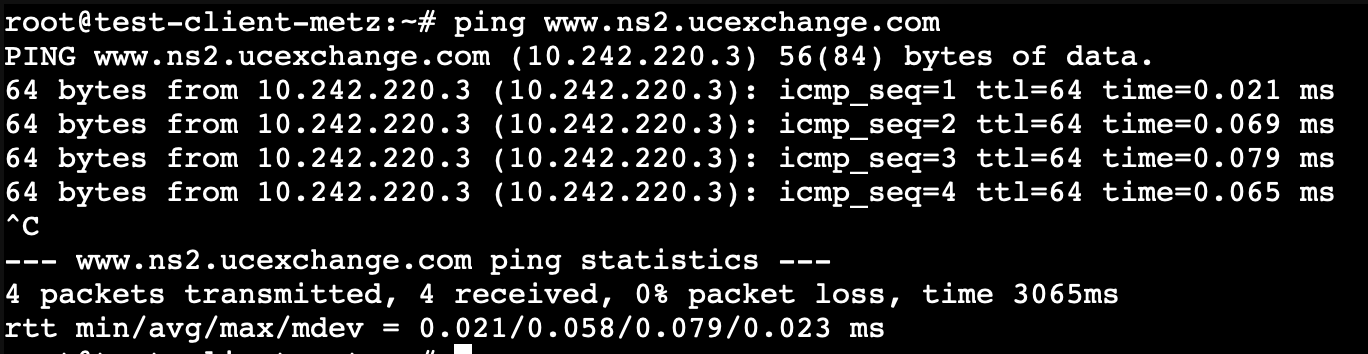
\includegraphics[width=0.9\textwidth]{img/web.png}
    \caption{Ping vers le serveur Web}
    \label{fig:web}
\end{figure}

Nous avons bien une réponse suite aux ping vers le serveur. J'ai choisi d'héberger
mon serveur Apache sur la même VM que la où est héberger le DNS secondaire. J'ai donc
utilisé le DNS secondaire pour le nom de domaine. C'est pourquoi nous avons 
en retour l'adresse IP de mon DNS secondaire et comme nom de domaine mon deuxième
DNS. 

\section{Conclusion}

En conclusion, le serveur DHCP, le serveur Web Apache et la 
configuration de DNS avec Bind9 sont des composants importants 
d'un réseau informatique. Le serveur DHCP simplifie la gestion des 
adresses IP sur un réseau en attribuant automatiquement des adresses 
IP aux dispositifs connectés. Le serveur Web Apache permet de publier 
et de gérer des sites Web tandis que la configuration de DNS avec Bind9 
garantit la résolution efficace des noms de domaines en adresses IP.\\

Cette SAE m'a permis d'apprendre pas mal de choses sur la gestion de DNS et 
un serveur DHCP dont je ne connaissais pas l'existence. J'ai pu aussi décvourvrir
comment le coeur d'un réseau informatique fonctionnait au sein d'une entreprise
présente sur plusieurs sites. Avec mes camarades nous avons même résusi à 
interconnecter les 3 parties, pour que la partie LAN puisse prendre des adresses
IP depuis mon serveur DHCP, et pour que la partie FAI puisse faire communiquer le site 
de Strasboug avec le site de Metz.

\end{document}